% \begin{document}
\chapter{Complessità Strutturale}

Finora abbiamo studiato le classi $RE$ e $R$, occupandoci di stabilire se un problema fosse decidibile o meno. D'ora in poi ci concentreremo esclusivamente sui problemi $\in R$, ovvero sui problemi \textit{decidibili}, e ci chiederemo quanto siano \textit{difficili} tra loro.

Questa area di ricerca nasce da una questione storica e tecnologica: negli anni '30, con Turing, tutto era molto astratto. La domanda era ``se mai fossi in grado di costruire questa macchina, che problemi sarebbe in grado di risolvere?''. Quando nei primi anni '60 le macchine reali arrivarono, la gente si trovava lì ad aspettare le risposte e si rese conto che certi problemi richiedevano molto più tempo di altri. Nacque allora la domanda fondamentale:

\begin{center}
\textit{``L'algoritmo che ho è lento perché non sono furbo a sufficienza, o il problema è talmente complicato che non riuscirò mai ad avere un algoritmo veloce?''}
\end{center}

Questo fu formalizzato da \textbf{Hartmanis, Stearns e Lewis nel 1965}, introducendo i concetti di \textbf{complessità temporale} e \textbf{complessità spaziale}. Lo studio si chiama \textbf{complessità strutturale} perché si vuole occupare della struttura dei problemi:

\begin{center}
\textit{``Com'è che la struttura di un problema influenza la complessità degli algoritmi che lo risolvono?''}
\end{center}

L'oggetto di interesse non è la complessità di un algoritmo specifico (come nel corso di Algoritmi e Strutture Dati), bensì la complessità \textit{intrinseca del problema}, indipendentemente dall'algoritmo scelto:

\begin{center}
\textit{Dato un problema, stabilire la famiglia di problemi di complessità simile a cui appartiene.}
\end{center}

\section{Definizioni di Complessità Temporale}

Ci focalizzeremo sull'insieme dei problemi decidibili. L'obiettivo è arricchire la struttura di $R$ identificando al suo interno classi di linguaggi di difficoltà differente.

\dfn{Computation Time}{
  Si definisce \textit{computation time} di una MdT $M$ su input $w$ il numero di passi che $M$ esegue prima di arrestarsi su $w$.\\
  Se $M$ è non deterministica, il computation time è dato dalla lunghezza del \textit{branch di computazione più lungo} nell'albero delle computazioni.
}

\dfn{Time Function}{
  Si definisce \textit{time function} una funzione $t : \mathbb{N} \to \mathbb{N}$ tale che $t(n)$ è non decrescente e strettamente positiva.
}

\dfn{Running Time}{
  Sia $t(n)$ una time function. Si definisce il \textit{running time} di una MdT $M$ pari a $t(n)$ se per tutte le stringhe $w$, a parte un numero finito, il computation time di $M$ su $w$ non eccede $t(\|w\|)$.
}

\nt{
  L'eccezione per un numero finito di stringhe serve a non far dipendere la definizione da casi limite irrilevanti: ci interessa il comportamento asintotico, non gli outlier.
}

\subsection{Notazione Asintotica}

\dfn{Big O}{
  Si definisce \textit{Big O}: una funzione $f(n) \in O(g(n))$ per un'altra funzione $g(n)$ se:
  \[
    \exists\, c, n_0 \;:\; \forall n \geq n_0,\quad f(n) \leq c \cdot g(n)
  \]
  Rappresenta un \textit{limite asintotico superiore}.
}

\dfn{Big $\Omega$}{
  Si definisce \textit{Big Omega}: una funzione $f(n) \in \Omega(g(n))$ per un'altra funzione $g(n)$ se:
  \[
    \exists\, c, n_0 \;:\; \forall n \geq n_0,\quad f(n) \geq c \cdot g(n)
  \]
  Rappresenta un \textit{limite asintotico inferiore}.
}

\dfn{Big $\Theta$}{
  Si definisce \textit{Big Theta}: una funzione $f(n) \in \Theta(g(n))$ se $f(n) \in O(g(n))$ e $f(n) \in \Omega(g(n))$ simultaneamente. Rappresenta un \textit{limite asintotico stretto}.
}

\subsection{Complessità di un Problema}

Attraverso la notazione asintotica introduciamo il concetto centrale di complessità di un \textit{problema}, distinguendola dalla complessità di un algoritmo specifico.

\dfn{Time Complexity Upper Bound}{
  Si definisce il \textit{time complexity upper bound} di un problema $P$ pari a $O(f(n))$ (dove $f(n)$ è una time function) se esiste almeno una MdT che risolve $P$ con un running time che è $O(f(n))$.
}

\dfn{Time Complexity Lower Bound}{
  Si definisce il \textit{time complexity lower bound} di un problema $P$ pari a $\Omega(f(n))$ (dove $f(n)$ è una time function) se \textbf{tutti} gli algoritmi o tutte le MdT che risolvono $P$ hanno un running time che è $\Omega(f(n))$.
}

\nt{
  Questa è la distinzione concettuale più importante del capitolo. Il lower bound dice che nessun algoritmo, presente o futuro, potrà mai fare meglio di così. L'upper bound dice che esiste almeno un algoritmo che fa così bene. Quando i due limiti coincidono, conosciamo la complessità \textit{esatta} del problema.
}

\[
  \Rightarrow \text{la complessità temporale di un problema è legata alla complessità temp. degli algoritmi che lo risolvono.}
\]

\section{Classe DTime e la Classe P}

\dfn{Classe di Complessità Temporale DTime}{
  Sia $t(n)$ una time function. Si definisce la classe di complessità temporale deterministica:
  \[
    DTime(t(n)) = \left\{ L \;\middle|\; \exists\, M \text{ deterministica che \underline{decide} } L \text{ in tempo } O(t(n)) \right\}
  \]
}

\dfn{Classe P}{
  Si definisce la classe \textit{P} (Polynomial Time) come l'unione di tutte le classi $DTime$ con limite temporale polinomiale:
  \[
    P = \bigcup_{c \geq 1} DTime(n^c)
  \]
  $P$ identifica i problemi \textit{trattabili}: risolvibili in tempo polinomiale deterministico.
}

\nt{
  $P$ contiene solo \textit{problemi di decisione} (risposta sì/no). Conseguentemente, ``ordinare un array'' o ``sommare due numeri'' non sono elementi di $P$ in senso formale, perché non sono problemi di decisione. Le loro versioni decisionali (``esiste un elemento $> k$?'') invece appartengono a $P$.

  Inoltre, $P$ è \textbf{invariante rispetto ai modelli di calcolo deterministici ragionevoli}: simulare un modello avanzato su una MdT a nastro singolo, oppure su un computer RAM convenzionale, produce al massimo un incremento polinomiale nel tempo, assorbito dalla definizione stessa di $P$.
}

\subsection{Esempi in P}

\subsubsection{Reachability}

\[
  Reach = \left\{ \langle G, s, t \rangle \;\middle|\;
  \begin{array}{l}
    G \text{ è un grafo diretto,} \\
    s, t \text{ sono nodi } \in G, \\
    \exists \text{ un percorso da } s \text{ a } t \in G
  \end{array}
  \right\}
\]

$Reach \in P$: è sufficiente una BFS/DFS a partire da $s$. L'algoritmo visita ogni nodo al più una volta, con costo $O(n^2)$ nella taglia del grafo.

\subsubsection{Primes}

\[
  Primes = \{ n \mid n \text{ è un numero primo} \}
\]

L'algoritmo \textit{naive} — dividere $n$ per $2, 3, \ldots, n-1$ — sembra $O(n)$ divisioni, ma bisogna stare attenti a cosa intendiamo per ``taglia dell'input''. L'input è $n$ rappresentato in \textbf{binario}: ha taglia $\|n\| = \log_2 n$ bit. Quindi il valore $n \approx 2^{\|n\|}$, e il numero di divisioni è $O(2^{\|n\|})$: \textbf{esponenziale nella taglia dell'input}.

\[
  n \approx 2^{\|n\|} \implies \text{algoritmo naive}: O\!\left(2^{\|n\|} \cdot \|n\|^k\right)
\]

Nonostante questo, $Primes \in P$ dagli inizi del 2000: Agrawal, Kayal e Saxena (algoritmo \textbf{AKS}) hanno dimostrato l'esistenza di un algoritmo deterministico polinomiale, con complessità $O(n^6)$ nella taglia dell'input. Fu un risultato storico e sorprendente, atteso per decenni.

\ex{}{
  Il numero $N = 1.000.000$ richiede circa $\log_2(10^6) \approx 20$ bit per essere rappresentato. L'algoritmo naive compie $\approx 10^6 = 2^{20}$ divisioni: raddoppiare la taglia dell'input (da 10 a 20 bit) fa esplodere il numero di operazioni da $10^3$ a $10^6$. Questa è la definizione di crescita esponenziale rispetto alla taglia.
}

\section{Classe NTime e la Classe NP}

I seguenti due problemi resistono ad algoritmi polinomiali deterministici e motivano la definizione di una nuova classe.

\subsection{SAT (Soddisfacibilità Booleana)}

Ci interessano formule in \textbf{Forma Normale Congiuntiva (CNF)}: una congiunzione di clausole, dove ogni clausola è una disgiunzione di letterali.

\[
  \mathcal{C} = c_1 \wedge c_2 \wedge \cdots \wedge c_n, \qquad
  c_i = l_1 \vee l_2 \vee \cdots \vee l_m, \qquad
  l_j = x_k \;\text{ oppure }\; \neg x_k
\]

\ex{}{
  \[
    \mathcal{C} = (x_1 \vee x_2 \vee \neg x_3) \wedge (\neg x_2 \vee x_4) \wedge (\neg x_3 \vee x_5 \vee \neg x_6)
  \]
  Con l'assegnamento $x_1 = V,\; x_2 = F,\; x_5 = V$, la formula è soddisfatta.
}

\[
  Sat = \left\{ \varphi \;\middle|\; \varphi \text{ è in CNF e soddisfacibile} \right\}
\]

Dato un assegnamento in mano, verificare se soddisfa la formula costa tempo polinomiale: si scorrono tutte le clausole e si controlla che almeno un letterale per clausola sia vero.

Il problema è \textit{trovare} quell'assegnamento: con $n$ variabili ci sono $2^n$ assegnamenti possibili. Testarli tutti costa:
\[
  O\!\left(2^n \cdot \mathrm{poly}(\|\varphi\|)\right)
\]
Tempo esponenziale. Da ciò non possiamo concludere che $Sat \notin P$, semplicemente questo algoritmo non lo colloca in $P$.

\subsection{Independent Set}

\dfn{Independent Set}{
  Si definisce \textit{independent set} di un grafo $G$ un insieme $S$ di nodi tale che nessuna coppia di nodi in $S$ è collegata da un arco.
}

\[
  IS = \left\{ \langle G, k \rangle \;\middle|\; \exists \text{ un independent set di taglia } k \in G \right\}
\]

Dato un insieme $S$, verificare che sia un IS richiede tempo quadratico (si controllano tutte le coppie). Trovarlo richiede generare tutti i $\binom{n}{k}$ sottoinsiemi di taglia $k$:
\[
  \binom{n}{k} \cdot O(n^2) \quad \Rightarrow \text{ esponenziale}
\]

\subsection{L'intuizione non deterministica}

SAT e IS condividono un pattern:
\begin{enumerate}
  \item La difficoltà sta nel \textit{trovare} la soluzione (assegnamento, sottoinsieme).
  \item Una volta trovata, \textit{verificarla} è facile (polinomiale).
\end{enumerate}

Una \textbf{MdT non deterministica} sfrutta esattamente questo: invece di esplorare tutto lo spazio delle soluzioni, \textit{indovina} la soluzione giusta e poi la verifica. La macchina accetta se \textit{esiste almeno un ramo} dell'albero di computazione che accetta.

\ex{IS su MdT non deterministica}{
  \begin{enumerate}
    \item \textbf{Fase di guess}: per ogni nodo, la MdT ND sceglie non deterministicamente se includerlo in $S$ o meno. Costo $O(n)$.
    \item \textbf{Fase di check}: verifica che $|S| = k$ e che nessun arco colleghi due nodi in $S$. Costo $O(n^2)$.
  \end{enumerate}
  Complessivamente: tempo \textbf{polinomiale non deterministico}. Similmente per SAT: la MdT indovina un assegnamento in $O(n)$ e lo verifica in $O(\|\varphi\|)$.
}

\dfn{Classe di Complessità NTime}{
  Sia $t(n)$ una time function. Si definisce la classe di complessità temporale non deterministica:
  \[
    NTime(t(n)) = \left\{ L \;\middle|\; \exists\, M \text{ non deterministica che decide } L \text{ in tempo } O(t(n)) \right\}
  \]
}

\dfn{Classe NP}{
  Si definisce la classe \textit{NP} (Non-deterministic Polynomial Time) come:
  \[
    NP = \bigcup_{c \geq 1} NTime(n^c)
  \]
  $NP$ è la classe dei problemi la cui soluzione può essere \textbf{verificata} in tempo polinomiale, equivalentemente dei problemi \textbf{risolti} in tempo polinomiale non deterministico.
}

\nt{
  Dire che un problema è in $NP$ \textbf{non} significa che si riesce a risolverlo velocemente: significa che se qualcuno ci regala la soluzione (il \textit{certificato}), possiamo verificarla in tempo polinomiale. È questa l'intuizione del pattern \textit{Guess \& Check}.
}

\section{La Questione P vs NP}

Chiaramente $P \subseteq NP$: qualsiasi problema risolvibile deterministicamente in tempo polinomiale può anche essere verificato in tempo polinomiale. La domanda aperta fondamentale è:

\[
  \boxed{P \overset{?}{=} NP}
\]

Ovvero: ogni problema la cui soluzione è facilmente \textit{verificabile} è anche facilmente \textit{trovabile}? La risposta è quasi certamente no, ma non è mai stata dimostrata. È uno dei sette Millennium Prize Problems (Clay Mathematics Institute, 2000).

\nt{
  Un teorema centrale in questa direzione è il risultato di \textbf{Baker, Gill e Solovay (1975)}: esistono due oracoli $A$ e $B$ tali che $P^A = NP^A$ ma $P^B \neq NP^B$. Questo dimostra che qualsiasi tecnica di dimostrazione \textit{relativizzante} (come la diagonalizzazione pura) non potrà mai risolvere la questione P vs NP, poiché qualunque risultato ottenuto con tali tecniche dovrebbe valere per entrambi gli oracoli simultaneamente.
}

\begin{center}
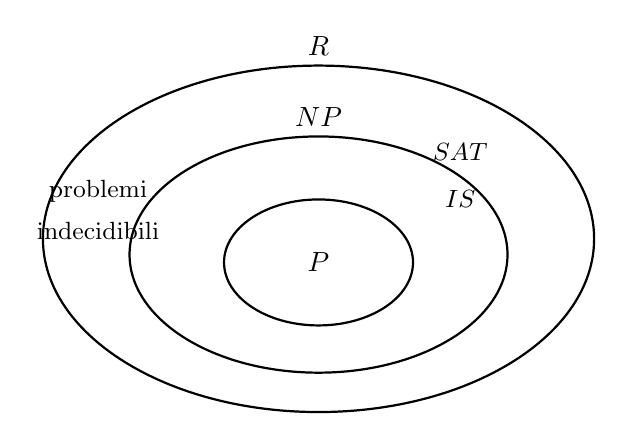
\begin{tikzpicture}
  \draw[thick] (0,0) ellipse (3.5cm and 2.2cm);
  \node[above] at (0, 2.2) {$R$};
  \draw[thick] (0,-0.2) ellipse (2.4cm and 1.5cm);
  \node[above] at (0, 1.3) {$NP$};
  \draw[thick] (0,-0.3) ellipse (1.2cm and 0.8cm);
  \node at (0,-0.3) {$P$};
  \node[font=\small] at (-2.8, 0.6) {problemi};
  \node[font=\small] at (-2.8, 0.1) {indecidibili};
  \node[font=\small] at (1.8, 1.1) {$SAT$};
  \node[font=\small] at (1.8, 0.5) {$IS$};
\end{tikzpicture}
\end{center}

\section{Riduzioni Polinomiali}
\dfn{Riduzione Polinomiale}{
  Siano $ A $ e $ B $ due linguaggi. Si dice che $ A $ si \textit{riduce polinomialmente} a $ B $ ($ A \leq_P B $) se $ \exists f: \Sigma^* \to \Sigma^* $ tale che:
  \begin{enumerate}
  \item $ f $ e' calcolabile in tempo polinomiale deterministico
  \item $ \forall w \in \Sigma^* $
    \[
      w \in A \iff f(w) \in B
    \]
  \end{enumerate}
}

\dfn{NP-Hardness}{
  Un linguaggio $ A $ si dice \textit{NP-Hard} se $ \forall L \in NP $
  \[
  L \leq_P A
  \]
}

\dfn{NP-Completeness}{
  Un linguaggio $ A $ si dice \textit{NP-Complete} se 
  \begin{enumerate}
  \item $ A $ e' NP-Hard
  \item $ A \in NP $
  \end{enumerate}
}

\thm{Collasso di NP}{
  Sia $ L $ un linguaggio NP-Complete, allora
  \[
  L \in P \iff P = NP
  \]
}
\pf{Dimostrazione}{
  \begin{itemize}
    \item $ \impliedby) $ Abbiamo che $ L \in NP $ dato che e' NP-Complete, ma per ipotesi $ NP = P $ quindi $ L \in P $.
    \item $ \implies) $ Dato che $ L $ e' NP-Complete sappiamo che tutti i linguaggi NP si riducono polinomialmente a $ L $. Ma per ipotesi $ L $ e' risolvibile in tempo polinomiale deterministico, quindi anche tutti i linguaggi che si riducono polinomialmente a esso appartengono a $ P $, quindi $ NP \subseteq P $. Se un problema e' risolvibile con una macchina deterministica, allora esiste sicuramente una macchina non deterministica che lo risolve, quindi $ P \subseteq NP $. Quindi $ P = NP $.  
  \end{itemize}
}

\thm{Transitivita' delle riduzioni polinomiali}{
  Siano $ A,B $ e $ C $ tre linguaggi. Se $ A \leq_P B $ e $ B \leq_P C $, allora
  \[
  A \leq_P C
  \]
}
\pf{Dimostrazione}{
  Basta considerare la composizione delle funzioni garantite dalla riduzione. Dato che queste sono deterministiche polinomiali, lo sara' anche la composizione.
}

\thm{Riduzioni NP-Hard}{
  Dati due linugaggi $ A,B $ con $ A $ NP-Hard tali che $ A \leq_P B $, allora
  \[
    B \text{e' NP-Hard} 
  \]
}
\pf{Dimostrazione}{
  Sfruttiamo la transitivita' della riduzione polinomiale per dimostrare che se $ \forall L \in NP. L \leq_P A $ e $ A \leq_P B $ allora $ B $ e' NP-Hard.
}

Useremo questa proprieta' per dimostrare che un linugaggio e' NP-Hard, dato che trovare una riduzione per ogni linugaggio in NP e' impossibile (ce ne stanno infiniti). Ci serve pero' almeno un linugaggio che sappiamo essere NP-Hard verso il quale ci possiamo ridurre, e questo e' proprio SAT (vedremo piu' avanti come si puo' dimostrare). Per facilitarci la vita useremo un linugaggio simile, 3SAT, che dimostriamo essere NP-Hard riducendoci SAT

\dfn{3SAT}{
  Come SAT, ma le formule sono in 3CNF (ogni clausola $ c_i $ ha lunghezza massima di 3 letterali)
  \[
  \text{3STA} = \{\psi | \psi \text{ e' in 3CNF ed e' soddisfacibile}\}
  \]
}

\mprop{NP-Completezza di 3SAT}{
  3SAT e' NP-Completo
}
\pf{Dimostrazione}{
  \textbf{3SAT $\in$ NP}: il certificato e' un'assegnazione; la verifica che ogni clausola
  abbia un letterale vero e' polinomiale.

  \textbf{$\text{SAT} \leq_P \text{3SAT}$}: data $\phi$ in CNF, costruiamo $\phi'$ in 3CNF
  tale che $\phi \text{ soddisfacibile} \iff \phi' \text{ soddisfacibile}$.
  Per ogni clausola $C_i = (l_1 \vee \cdots \vee l_k)$:
  \begin{itemize}
    \item \textbf{$k = 1$:} si aggiungono due variabili fresche $y_1, y_2$ e si sostituisce con:
      \[
        (l_1 \vee y_1 \vee y_2)\wedge(l_1 \vee y_1 \vee \neg y_2)\wedge(l_1 \vee \neg y_1 \vee y_2)\wedge(l_1 \vee \neg y_1 \vee \neg y_2)
      \]
    \item \textbf{$k = 2$:} si aggiunge una variabile fresca $y$ e si sostituisce con:
      \[
        (l_1 \vee l_2 \vee y)\wedge(l_1 \vee l_2 \vee \neg y)
      \]
    \item \textbf{$k = 3$:} invariata.
    \item \textbf{$k > 3$:} si introducono $k-3$ variabili fresche $z_1,\dots,z_{k-3}$ e si sostituisce con la catena:
      \[
        (l_1 \vee l_2 \vee z_1)\wedge(\neg z_1 \vee l_3 \vee z_2)\wedge\cdots\wedge(\neg z_{k-3} \vee l_{k-1} \vee l_k)
      \]
  \end{itemize}

  La riduzione e' polinomiale: ogni clausola di $k$ letterali produce $O(k)$ clausole e variabili.

  \textbf{Completezza} ($\phi$ soddisfacibile $\Rightarrow$ $\phi'$ soddisfacibile):
  \begin{itemize}
    \item Sia $l_{i^*} = \top$ il letterale vero in $C_i$.
    \item Si pone $z_j = \top$ per $j < i^*-2$, $z_j = \bot$ per $j \geq i^*-2$.
    \item Le clausole prima di $i^*$ sono soddisfatte da $z_j = \top$, quella in $i^*$ da $l_{i^*} = \top$, quelle dopo da $\neg z_j = \top$.
  \end{itemize}

  \textbf{Correttezza} ($\phi'$ soddisfacibile $\Rightarrow$ $\phi$ soddisfacibile),
  per assurdo supponiamo $l_j = \bot$ per ogni $j$:
  \begin{itemize}
    \item $(l_1 \vee l_2 \vee z_1)$: $l_1 = l_2 = \bot \Rightarrow z_1 = \top$.
    \item Per induzione: $z_j = \top$ e $l_{j+2} = \bot \Rightarrow z_{j+1} = \top$.
    \item Ma nell'ultima clausola $(\neg z_{k-3} \vee l_{k-1} \vee l_k)$: tutti $\bot$. Contraddizione.
  \end{itemize}
}

\section{Independent Set, Vertex Cover e Clique}

La catena di riduzioni che costruiremo e':
\[
  \text{3SAT} \leq_P \text{IS} \leq_P \text{VC}, \qquad \text{IS} \leq_P \text{CLIQUE}
\]

\subsection{Independent Set}

\dfn{Independent Set (problema decisionale)}{
  \[
    \text{IS} = \{\langle G, k \rangle \mid G \text{ ha un independent set } S \text{ con } |S| \geq k\}
  \]
  dove un independent set e' un $S \subseteq V$ tale che nessuna coppia di nodi in $S$ e' collegata da un arco.
}

\thm{NP-Completezza di IS}{
  IS e' NP-Completo.
}
\pf{Dimostrazione}{
  \textbf{IS $\in$ NP}: guess \& check. Una NTM genera $S \subseteq V$, verifica $|S| \geq k$ e che $\forall u,v \in S.\; \{u,v\} \notin E$. Costo $O(|S|^2)$.

  \textbf{$\text{3SAT} \leq_P \text{IS}$}: data $\varphi = C_1 \wedge \cdots \wedge C_m$ in 3CNF su variabili $x_1,\dots,x_n$, costruiamo $\langle G, k \rangle$ con $k = m$:

  \begin{itemize}
    \item \textbf{Nodi}: per ogni \textit{occorrenza} di letterale nella formula, un nodo. Totale $3m$ nodi, raggruppati in $m$ triangoli (uno per clausola).
    \item \textbf{Archi intra-clausola}: si collegano i 3 nodi di ogni clausola a formare un triangolo. $\Rightarrow$ da ogni clausola al piu' un nodo nell'IS.
    \item \textbf{Archi inter-clausola (consistenza)}: si aggiunge un arco tra ogni coppia di nodi etichettati con letterali complementari ($x_i$ e $\neg x_i$ in clausole diverse). $\Rightarrow$ impossibile selezionare un letterale e la sua negazione.
  \end{itemize}

  \textbf{Completezza} ($\varphi$ soddisfacibile $\Rightarrow$ IS di taglia $\geq k$):
  \begin{itemize}
    \item Dall'assegnamento $\tau \models \varphi$, per ogni clausola $C_j$ scegliamo un letterale vero $\ell^{C_j}$ e lo mettiamo in $S$.
    \item $|S| = m = k$, un nodo per triangolo $\Rightarrow$ nessun arco intra-clausola violato.
    \item $\tau$ e' consistente $\Rightarrow$ nessun arco inter-clausola violato.
  \end{itemize}

  \textbf{Correttezza} (IS di taglia $\geq k$ $\Rightarrow$ $\varphi$ soddisfacibile):
  \begin{itemize}
    \item $|S| \geq m$ con $m$ triangoli $\Rightarrow$ $S$ contiene esattamente un nodo per triangolo.
    \item Definiamo $\tau$: $x_i = \top$ se il nodo $x_i \in S$, $x_i = \bot$ se $\neg x_i \in S$, arbitrario altrimenti.
    \item Ben definito (no letterali complementari in $S$). Ogni clausola ha un letterale vero $\Rightarrow$ $\tau \models \varphi$.
  \end{itemize}

  La costruzione e' $O(m + n)$, quindi polinomiale.
}

\subsection{Vertex Cover}

\dfn{Vertex Cover (problema decisionale)}{
  \[
    \text{VC} = \{\langle G, k \rangle \mid G \text{ ha un vertex cover } C \text{ con } |C| \leq k\}
  \]
  dove un vertex cover e' un $C \subseteq V$ tale che per ogni arco $\{u,v\} \in E$, almeno uno tra $u$ e $v$ appartiene a $C$.
}

\nt{
  Intuitivamente: se gli archi sono corridoi e i nodi incroci, un vertex cover e' un posizionamento di telecamere agli incroci tale che ogni corridoio sia sorvegliato. L'obiettivo e' minimizzare il numero di telecamere.
}

\thm{Lemma del Complemento IS-VC}{
  Sia $G = (V,E)$ e $S \subseteq V$. Allora:
  \[
    S \text{ e' un IS di } G \iff V \setminus S \text{ e' un VC di } G
  \]
}
\pf{Dimostrazione}{
  Poniamo $C = V \setminus S$.

  \begin{itemize}
    \item $(\Rightarrow)$ $S$ e' un IS $\Rightarrow$ $C$ e' un VC.

    Sia $\{u,v\} \in E$ un arco qualsiasi. Dobbiamo mostrare che almeno un estremo sta in $C$.
    Poiche' $S$ e' un IS, $u$ e $v$ non possono stare \textit{entrambi} in $S$ (altrimenti sarebbero due nodi adiacenti nell'IS). Quindi almeno uno dei due $\notin S$, e di conseguenza $\in C = V \setminus S$. L'arco e' coperto.
    Questo vale per ogni arco, dunque $C$ e' un VC.

    \item $(\Leftarrow)$ $C$ e' un VC $\Rightarrow$ $S$ e' un IS.

    Siano $u,v \in S$ due nodi qualsiasi. Dobbiamo mostrare che $\{u,v\} \notin E$.
    Poiche' $u,v \in S = V \setminus C$, abbiamo $u,v \notin C$.
    Se per assurdo $\{u,v\} \in E$, questo arco non avrebbe nessun estremo in $C$: contraddizione col fatto che $C$ e' un VC. Dunque $\{u,v\} \notin E$.
    Questo vale per ogni coppia in $S$, dunque $S$ e' un IS.
  \end{itemize}

}

\cor{}{
  $G$ ha un IS di taglia $k$ $\iff$ $G$ ha un VC di taglia $|V| - k$.
}

\thm{NP-Completezza di VC}{
  VC e' NP-Completo.
}
\pf{Dimostrazione}{
  \textbf{VC $\in$ NP}: guess \& check. NTM genera $C \subseteq V$, verifica $|C| \leq k$ e che ogni arco abbia almeno un estremo in $C$.

  \textbf{$\text{IS} \leq_P \text{VC}$}: data $\langle G, k \rangle$ istanza di IS, costruiamo $\langle H, \ell \rangle$ con:
  \[
    H = G, \quad \ell = |V| - k
  \]
  \begin{itemize}
    \item $\langle G, k \rangle \in \text{IS}$: esiste IS $S$ con $|S| \geq k$. Per il lemma, $V \setminus S$ e' VC con $|V \setminus S| \leq |V| - k = \ell$. Dunque $\langle H, \ell \rangle \in \text{VC}$.
    \item $\langle H, \ell \rangle \in \text{VC}$: esiste VC $C$ con $|C| \leq \ell$. Per il lemma, $V \setminus C$ e' IS con $|V \setminus C| \geq k$. Dunque $\langle G, k \rangle \in \text{IS}$.
  \end{itemize}
  La riduzione non modifica il grafo, solo il parametro: $O(1)$.
}

\subsection{Clique}

\dfn{Clique (problema decisionale)}{
  \[
    \text{CLIQUE} = \{\langle G, k \rangle \mid G \text{ ha una clique } C \text{ con } |C| \geq k\}
  \]
  dove una clique e' un $C \subseteq V$ tale che ogni coppia $u,v \in C$ e' collegata: $\{u,v\} \in E$.
}

\dfn{Grafo Complemento}{
  Dato $G = (V,E)$, il complemento $\bar{G} = (V, \bar{E})$ ha:
  \[
    \bar{E} = \{\{u,v\} \mid u \neq v,\; \{u,v\} \notin E\}
  \]
}

\thm{Lemma del Complemento IS-Clique}{
  Sia $G = (V,E)$ e $S \subseteq V$. Allora:
  \[
    S \text{ e' un IS di } G \iff S \text{ e' una clique di } \bar{G}
  \]
}
\pf{Dimostrazione}{
  $(\Rightarrow)$ $S$ e' un IS di $G$ $\Rightarrow$ $S$ e' una clique di $\bar{G}$.

  Siano $u,v \in S$ due nodi qualsiasi. Poiche' $S$ e' un IS di $G$, i nodi $u$ e $v$ non sono adiacenti in $G$: $\{u,v\} \notin E$. Ma per definizione di grafo complemento, se un arco non esiste in $G$ allora esiste in $\bar{G}$: $\{u,v\} \in \bar{E}$.
  Questo vale per ogni coppia in $S$, dunque tutti i nodi di $S$ sono mutualmente collegati in $\bar{G}$: $S$ e' una clique.

  $(\Leftarrow)$ $S$ e' una clique di $\bar{G}$ $\Rightarrow$ $S$ e' un IS di $G$.

  Siano $u,v \in S$ due nodi qualsiasi. Poiche' $S$ e' una clique di $\bar{G}$, i nodi $u$ e $v$ sono adiacenti in $\bar{G}$: $\{u,v\} \in \bar{E}$. Ma per definizione di grafo complemento, se un arco esiste in $\bar{G}$ allora non esiste in $G$: $\{u,v\} \notin E$.
  Questo vale per ogni coppia in $S$, dunque nessun nodo di $S$ e' collegato ad un altro in $G$: $S$ e' un IS.
}

\thm{NP-Completezza di CLIQUE}{
  CLIQUE e' NP-Completo.
}
\pf{Dimostrazione}{
  \textbf{CLIQUE $\in$ NP}: guess \& check. NTM genera $C \subseteq V$, verifica $|C| \geq k$ e che ogni coppia sia collegata.

  \textbf{$\text{IS} \leq_P \text{CLIQUE}$}: data $\langle G, k \rangle$ istanza di IS, costruiamo:
  \[
    H = \bar{G}, \quad \ell = k
  \]
  \begin{itemize}
    \item $\langle G, k \rangle \in \text{IS}$: esiste IS $S$ con $|S| \geq k$. Per il lemma, $S$ e' clique di $\bar{G} = H$. Dunque $\langle H, \ell \rangle \in \text{CLIQUE}$.
    \item $\langle H, \ell \rangle \in \text{CLIQUE}$: esiste clique $C$ di $\bar{G}$ con $|C| \geq k$. Per il lemma, $C$ e' IS di $G$. Dunque $\langle G, k \rangle \in \text{IS}$.
  \end{itemize}
  Costruzione di $\bar{G}$: $O(|V|^2)$, polinomiale.
}

\section{Dominating Set e Kernel}

\subsection{Dominating Set}

\dfn{Dominating Set}{
  Dato $G = (V,E)$ non diretto, un \textit{dominating set} e' un $D \subseteq V$ tale che per ogni $v \in V \setminus D$ esiste $u \in D$ con $\{u,v\} \in E$. In altre parole, $D$ ``domina'' tutto il resto del grafo: ogni nodo fuori da $D$ e' raggiungibile da $D$ in un singolo salto.
  \[
    \text{DS} = \{\langle G, k \rangle \mid G \text{ ha un dominating set } D \text{ con } |D| \leq k\}
  \]
}

E' importante non confondere DS con VC. In un Vertex Cover vogliamo coprire tutti gli \textit{archi} (ogni arco ha almeno un estremo nel cover); in un Dominating Set vogliamo raggiungere tutti i \textit{nodi} (ogni nodo fuori dal set ha un vicino nel set). Un VC e' sempre un DS in grafi senza nodi isolati, ma il viceversa non vale: un DS puo' ``saltare'' un arco intero, purche' entrambi gli estremi siano dominati da qualche altro nodo.

\thm{NP-Completezza di DS}{
  DOMINATING SET e' NP-Completo.
}
\pf{Dimostrazione}{
  \textbf{DS $\in$ NP}: indovino un insieme $D$ di taglia $\leq k$ e verifico che ogni nodo fuori da $D$ abbia almeno un vicino dentro $D$. Guess e check entrambi in tempo polinomiale.

  \textbf{$\text{VC} \leq_P \text{DS}$}: non possiamo usare $H = G$ direttamente perche' un DS non implica necessariamente un VC. La costruzione e' piu' furba.

  Data $\langle G, k \rangle$ istanza di VC (senza nodi isolati), costruiamo $H$ aggiungendo un nuovo nodo per ogni arco di $G$: se $G$ ha un arco $e = \{u,v\}$, aggiungiamo in $H$ un nodo $v_e$ collegato sia a $u$ che a $v$ (e a nient'altro). La soglia resta $\ell = k$.

  \textbf{Completezza} ($G$ ha VC $C$ con $|C| \leq k$ $\Rightarrow$ $H$ ha DS di taglia $\leq k$):

  Mostriamo che $C$ e' gia' un DS di $H$. Per ogni nodo originale $v \notin C$: poiche' $G$ non ha nodi isolati, $v$ ha almeno un vicino, e quell'arco e' coperto da $C$, quindi almeno un vicino di $v$ sta in $C$ -- $v$ e' dominato. Per ogni nodo speciale $v_e$ (aggiunto per $e = \{u,v\}$): per definizione di VC, almeno uno tra $u$ e $v$ sta in $C$, ed e' adiacente a $v_e$ in $H$ -- $v_e$ e' dominato. Dunque $C$ e' un DS di $H$ di taglia $\leq k$.

  \textbf{Correttezza} ($H$ ha DS $D$ con $|D| \leq k$ $\Rightarrow$ $G$ ha VC di taglia $\leq k$):

  $D$ potrebbe contenere nodi speciali. Li sostituiamo: per ogni $v_e \in D$ (nodo aggiunto per l'arco $\{u,v\}$), lo rimpiazziamo con uno degli estremi $u$ o $v$. Il nodo $v_e$ era collegato solo a $u$ e $v$, quindi dominava al piu' loro; sostituirlo con $u$ (o $v$) mantiene la dominanza su tutti i nodi vicini. La taglia non aumenta.

  Dopo la sostituzione, $D$ contiene solo nodi originali di $G$. Poiche' $D$ deve dominare ogni nodo speciale $v_e$, deve contenere almeno uno tra $u$ e $v$ per ogni arco $\{u,v\}$: questa e' esattamente la definizione di vertex cover. Dunque $D$ e' un VC di $G$ di taglia $\leq k$.

  Costruzione: $O(|V| + |E|)$, polinomiale.
}

\subsection{Kernel}

\dfn{Kernel}{
  Dato un grafo \textbf{diretto} $G = (V,E)$, un \textit{kernel} e' un $K \subseteq V$ che soddisfa simultaneamente:
  \begin{enumerate}
    \item \textbf{Indipendenza}: $K$ e' un IS di $G$ -- non esistono $u,v \in K$ con $(u,v) \in E$.
    \item \textbf{Dominanza (assorbenza)}: per ogni $v \in V \setminus K$, esiste $u \in K$ con $(v, u) \in E$ -- ogni nodo esterno ha un arco \textit{uscente} verso un nodo del kernel.
  \end{enumerate}
  \[
    \text{KERNEL} = \{G \mid G \text{ e' un grafo diretto che possiede un kernel}\}
  \]
}

\nt{
  La proprieta' di dominanza e' simile al dominating set, ma orientata: non basta essere adiacenti, ci deve essere un arco che va \textit{dal} nodo esterno \textit{verso} $K$. Notare anche che non c'e' un parametro $k$: si chiede solo l'esistenza di un kernel, di qualsiasi taglia. Il problema e' gia' difficile senza vincoli sulla taglia.

  Il kernel modella le ``posizioni vincenti'' in un gioco combinatorio a due giocatori: se ti trovi su un nodo del kernel, il tuo avversario e' costretto a muoversi fuori dal kernel; da fuori, puoi sempre tornare nel kernel al prossimo passo.
}

\thm{NP-Completezza di KERNEL}{
  KERNEL e' NP-Completo.
}
\pf{Dimostrazione}{
  \textbf{KERNEL $\in$ NP}: indovino un insieme $K$, verifico che sia indipendente (nessun arco tra nodi di $K$) e assorbente (ogni nodo esterno ha un arco verso $K$). Entrambe le verifiche in tempo polinomiale.

  \textbf{$\text{3SAT} \leq_P \text{KERNEL}$}: data $\varphi = C_1 \wedge \cdots \wedge C_m$ in 3CNF su variabili $x_1,\dots,x_n$, costruiamo un grafo diretto $G$ tale che $\varphi$ e' soddisfacibile $\iff$ $G$ ha un kernel.

  \textbf{Costruzione di $G$}:
  \begin{itemize}
    \item \textbf{Gadget variabile}: per ogni variabile $x_i$, creiamo due nodi $x_i$ e $\neg x_i$ collegati bidirezionalmente ($x_i \leftrightarrow \neg x_i$). In qualsiasi kernel: l'indipendenza impedisce che entrambi stiano in $K$; la dominanza impone che almeno uno ci stia (ciascuno dei due deve poter raggiungere qualcuno in $K$, e l'unico candidato e' il complementare). Quindi esattamente uno tra $x_i$ e $\neg x_i$ appartiene a $K$ -- questo corrisponde all'assegnamento della variabile.
    \item \textbf{Nodi clausola}: per ogni clausola $C_j$, creiamo un nodo $C_j$.
    \item \textbf{Archi clausola $\to$ letterale}: per ogni letterale $\ell$ in $C_j$, arco $C_j \to \ell$. Cosi' il nodo clausola puo' ``raggiungere'' i letterali che la compongono: se almeno uno sta in $K$, allora $C_j$ e' dominato.
    \item \textbf{Archi letterale negato $\to$ clausola}: per ogni letterale $\ell$ in $C_j$, arco $\bar{\ell} \to C_j$. Questi archi servono a garantire la struttura corretta nella direzione inversa.
  \end{itemize}

  \textbf{Completezza} ($\varphi$ soddisfacibile $\Rightarrow$ $G$ ha un kernel):

  Dato $\tau \models \varphi$, costruiamo $K$ mettendo in $K$ il letterale vero di ogni coppia: $x_i \in K$ se $\tau(x_i) = \top$, $\neg x_i \in K$ altrimenti. I nodi clausola non entrano in $K$.

  $K$ e' indipendente: all'interno di ogni coppia $(x_i, \neg x_i)$ scegliamo un solo nodo. Tra nodi letterali di coppie diverse non ci sono archi. Nessun arco tra nodi di $K$.

  $K$ e' assorbente: ogni nodo letterale non in $K$ (diciamo $\neg x_i$, se $x_i \in K$) ha l'arco $\neg x_i \to x_i$ verso $K$, quindi e' dominato. Ogni nodo clausola $C_j$: poiche' $\tau \models \varphi$, almeno un letterale $\ell$ di $C_j$ e' vero, quindi $\ell \in K$, e l'arco $C_j \to \ell$ domina $C_j$.

  \textbf{Correttezza} ($G$ ha un kernel $K$ $\Rightarrow$ $\varphi$ e' soddisfacibile):

  In ogni coppia $(x_i, \neg x_i)$ esattamente uno sta in $K$ (come argomentato sopra), quindi l'assegnamento $\tau_K$ e' ben definito e consistente.

  I nodi clausola non possono stare in $K$: hanno archi uscenti verso nodi letterali che a loro volta sono collegati tra loro -- la struttura del gadget variabile impedirebbe l'indipendenza. Quindi ogni $C_j \notin K$, e per la dominanza deve esistere un arco $C_j \to \ell$ con $\ell \in K$. Ma i letterali in $K$ sono quelli resi veri da $\tau_K$, quindi $C_j$ contiene almeno un letterale vero: $\tau_K \models \varphi$.

  Costruzione: $O(n + m)$, polinomiale.
}

\section{Definizione Alternativa della Classe NP}

Guardando tutti i problemi NP studiati finora -- IS, VC, Clique, DS, 3SAT -- c'e' un pattern ricorrente. Per dimostrare che un problema $L$ sta in NP costruiamo sempre la stessa struttura:
\begin{enumerate}
  \item \textbf{Guess}: indoviniamo non deterministicamente una soluzione candidata
  \item \textbf{Check}: verifichiamo in tempo polinomiale deterministico che sia corretta
\end{enumerate}
In IS: indovino un insieme $S$, verifico che sia indipendente e abbia taglia $\geq k$. In 3SAT: indovino un assegnamento $\sigma$, verifico che soddisfi tutte le clausole. La domanda e': questo e' un caso, o riflette qualcosa di strutturale su NP?

La risposta e' che non e' un caso -- e' una caratterizzazione equivalente della classe NP. Questa e' la \textbf{definizione alternativa di NP tramite certificati}.

\subsection{Relazione Binaria e Certificati}

Per formalizzare l'idea di ``soluzione candidata'' e ``verifica'' usiamo il concetto di relazione binaria.

\dfn{Relazione Binaria}{
  Una relazione binaria $R$ su $\Sigma^*$ e' un insieme $R \subseteq \Sigma^* \times \Sigma^*$, cioe' un insieme di coppie di stringhe. La prima componente $x$ e' l'\textit{istanza del problema}, la seconda $y$ e' il \textit{certificato}.
}

\ex{}{
  Per IS: $x = \langle G, k \rangle$, $y = S$ (l'insieme di nodi). La coppia $\langle x, y \rangle \in R_{\text{IS}}$ se e solo se $S$ e' effettivamente un IS di taglia $\geq k$ in $G$. La relazione ``certifica'' le istanze si' di IS: $x \in \text{IS}$ se e solo se $\exists\, y$ tale che $\langle x, y \rangle \in R_{\text{IS}}$.
}

Perche' l'idea funzioni, la relazione deve soddisfare due proprieta':

\dfn{Polinomialmente Bilanciata}{
  $R$ e' \textit{polinomialmente bilanciata} se esiste una costante $c$ tale che per ogni $\langle x, y \rangle \in R$:
  \[
    \|y\| \leq \|x\|^c
  \]
  Il certificato non e' troppo piu' grande dell'istanza -- al piu' polinomialmente. Se il certificato fosse di taglia esponenziale, non potremmo nemmeno leggerlo in tempo polinomiale.
}

\dfn{Polinomialmente Decidibile}{
  $R$ e' \textit{polinomialmente decidibile} se esiste una MdT deterministica che, data una coppia $\langle x, y \rangle$, stabilisce in tempo polinomiale se appartiene a $R$.

  Dato il certificato, possiamo controllarne la correttezza in tempo polinomiale.
}

\subsection{Il Teorema Centrale}

\thm{Caratterizzazione di NP tramite certificati}{
  \[
    L \in NP \iff \exists\, R_L \text{ pol. bilanciata e pol. decidibile tale che } L = \{x \mid \exists\, y : \langle x, y \rangle \in R_L\}
  \]
}
\pf{Dimostrazione}{
  \textbf{($\Leftarrow$) Da $R_L$ a NP.}

  Supponiamo che esista $R_L$ polinomialmente bilanciata e decidibile con $L = \{x \mid \exists\, y : \langle x, y \rangle \in R_L\}$. Costruiamo una MdT non deterministica $M$ che decide $L$ in tempo polinomiale:
  \begin{enumerate}
    \item Dato $x$ in input, $M$ indovina non deterministicamente una stringa $y$ di lunghezza al piu' $\|x\|^c$ (possibile per il bilanciamento).
    \item $M$ verifica deterministicamente se $\langle x, y \rangle \in R_L$ usando il decisore polinomiale di $R_L$.
    \item Se si', accetta; altrimenti rifiuta.
  \end{enumerate}
  Se $x \in L$, esiste un $y$ tale che $\langle x, y \rangle \in R_L$: un ramo non deterministico indovinera' quel $y$ e la verifica dara' esito positivo. Se $x \notin L$, nessun $y$ funziona, nessun ramo accetta. Il tutto in tempo polinomiale, quindi $L \in NP$.

  \textbf{($\Rightarrow$) Da NP a $R_L$.}

  Supponiamo $L \in NP$: esiste una MdT non deterministica $M$ che decide $L$ in tempo $p(n)$. L'idea e' usare come certificato la \textbf{sequenza delle Instantaneous Description} (ID) del ramo accettante di $M$.

  Poiche' $M$ lavora in tempo $p(n)$, il ramo accettante e' una sequenza di al piu' $p(n)$ configurazioni, ciascuna di taglia $\leq p(n)$ (la macchina non puo' scrivere piu' di $p(n)$ simboli). Il certificato totale ha taglia $p(n) \cdot p(n)$ = prodotto di polinomi = ancora polinomiale.

  Il certificato $y$ = sequenza di ID del ramo accettante e':
  \begin{itemize}
    \item \textbf{Conciso}: taglia polinomiale in $\|x\|$ $\Rightarrow$ $R_L$ e' polinomialmente bilanciata.
    \item \textbf{Verificabile}: data la sequenza di ID, si verifica che ogni ID sia il legal successor della precedente secondo la funzione di transizione di $M$, e che l'ultima sia accettante. Questo si fa in tempo polinomiale deterministico $\Rightarrow$ $R_L$ e' polinomialmente decidibile.
  \end{itemize}

  Solo le istanze si' hanno un tale certificato: se $x \in L$ esiste un ramo accettante e quindi un certificato valido; se $x \notin L$ non esiste nessun ramo accettante e nessun certificato valido. Quindi $L$ e' caratterizzato da $R_L$ polinomialmente bilanciata e decidibile.
}

\subsection{Cosa ci dice questa caratterizzazione}

Il teorema ci da' una visione completamente nuova di NP:

\begin{center}
  \textit{NP = classe dei problemi le cui istanze si' ammettono certificati concisi e polinomialmente verificabili.}
\end{center}

La distinzione tra P e NP si riformula cosi':
\begin{itemize}
  \item In $P$: problemi la cui soluzione si \textbf{calcola} in tempo polinomiale.
  \item In $NP$: problemi la cui soluzione si \textbf{verifica} in tempo polinomiale (una volta che ce la danno).
\end{itemize}

Verificare una soluzione e' apparentemente piu' facile che trovarla. La domanda $P \overset{?}{=} NP$ chiede se questa differenza e' reale o solo apparente.

\ex{Certificati per i problemi noti}{
  \begin{center}
  \begin{tabular}{l l l l}
    \textbf{Problema} & \textbf{Istanza $x$} & \textbf{Certificato $y$} & \textbf{Verifica} \\ \hline
    IS & $\langle G, k \rangle$ & insieme $S$ & $S$ e' IS e $|S| \geq k$? \\
    VC & $\langle G, k \rangle$ & insieme $C$ & $C$ copre tutti gli archi e $|C| \leq k$? \\
    3SAT & formula $\varphi$ & assegnamento $\sigma$ & $\sigma$ soddisfa tutte le clausole? \\
    Clique & $\langle G, k \rangle$ & insieme $S$ & $S$ e' clique e $|S| \geq k$? \\
  \end{tabular}
  \end{center}
  In ogni caso il certificato ha taglia polinomiale e la verifica e' polinomiale.
}

\section{Colorabilita' dei Grafi (Vertex Coloring)}

Il problema della colorabilita' dei grafi nasce dal celebre \textbf{problema dei quattro colori}: e' possibile colorare qualsiasi mappa geografica usando al piu' quattro colori, in modo che due regioni confinanti non abbiano mai lo stesso colore? (Risposta affermativa, dimostrata nel 1976 con l'ausilio di un computer.)

Modellando la mappa come un grafo -- dove ogni regione e' un nodo e due nodi sono collegati se le regioni condividono un confine -- il problema diventa: e' possibile assegnare a ciascun nodo uno tra $k$ colori, in modo che nodi adiacenti ricevano colori diversi? Le applicazioni spaziano dall'assegnazione di frequenze radio allo scheduling di esami all'allocazione di registri nei compilatori.

\dfn{$k$-colorazione e numero cromatico}{
  Data una $k$-colorazione di $G = (V,E)$ una funzione $f : V \to \{1,\dots,k\}$ tale che per ogni arco $\{u,v\} \in E$ si abbia $f(u) \neq f(v)$. Il \textit{numero cromatico} $\chi(G)$ e' il minimo $k$ per cui $G$ ammette una $k$-colorazione.
  \[
    \text{VCOL} = \{\langle G, k \rangle \mid G \text{ e' un grafo non diretto che ammette una } k\text{-colorazione}\}
  \]
}

\ex{}{
  Un grafo bipartito (senza cicli di lunghezza dispari) e' sempre 2-colorabile. Un ciclo di lunghezza dispari richiede almeno 3 colori. Un grafo completo $K_n$ richiede esattamente $n$ colori.
}

\thm{NP-Completezza di VCOL}{
  VCOL e' NP-Completo.
}
\pf{Dimostrazione}{
  \textbf{VCOL $\in$ NP}: guess \& check. Si indovina $f(v) \in \{1,\dots,k\}$ per ogni nodo ($O(n \log k)$ passi), poi si verificano tutti gli archi ($O(|E|)$ confronti).

  \textbf{$\text{3SAT} \leq_P \text{VCOL}$}: la riduzione costruisce sempre un grafo con $k = 3$ colori fissi, indipendentemente dalla formula. Dati $\varphi = C_1 \wedge \cdots \wedge C_m$ su variabili $x_1,\dots,x_n$, costruiamo $\langle G, 3 \rangle$.

  \textbf{Ingrediente 1 -- Triangolo di base $\{T, F, B\}$}:
  creiamo tre nodi $T$ (true), $F$ (false), $B$ (base) collegati a triangolo.

  \begin{center}
    \includegraphics[width=0.25\textwidth]{img/vcol-triangolo-base.png}
  \end{center}

  In qualsiasi 3-colorazione, $T$, $F$, $B$ ricevono tre colori distinti. Chiamiamo ``colore true'' il colore di $T$, ``colore false'' quello di $F$, ``colore base'' quello di $B$.

  \textbf{Ingrediente 2 -- Gadget variabile}: per ogni variabile $x_i$, creiamo due nodi $x_i$ e $\neg x_i$ con archi:
  \begin{itemize}
    \item $\{x_i, \neg x_i\}$ -- non possono avere lo stesso colore.
    \item $\{x_i, B\}$ e $\{\neg x_i, B\}$ -- nessuno dei due puo' avere il colore ``base''.
  \end{itemize}
  Dunque dei due colori rimasti (``true'' e ``false''), uno va a $x_i$ e l'altro a $\neg x_i$: \textbf{una 3-colorazione codifica automaticamente un assegnamento di verita'}.

  \textbf{Ingrediente 3 -- Gadget OR}: un sotto-grafo con due nodi di input e un nodo di output tale che:
  \[
    \text{output puo' essere ``true''} \iff \text{almeno un input e' ``true''}
  \]
  Il gadget e' un triangolo con due nodi intermedi. Se entrambi gli input sono ``false'', i nodi intermedi sono forzati a prendere ``true'' e ``base'', e l'output -- collegato a entrambi -- deve essere ``false''. Se almeno un input e' ``true'', i gradi di liberta' sono sufficienti per colorare l'output con ``true''.

  \begin{center}
    \includegraphics[width=0.3\textwidth]{img/vcol-gadget-or.png}
  \end{center}

  Una clausola $(l_1 \vee l_2 \vee l_3)$ si modella concatenando due gadget OR:
  \begin{enumerate}
    \item Primo gadget OR: input $l_1$ e $l_2$, output intermedio $= l_1 \vee l_2$.
    \item Secondo gadget OR: input $l_1 \vee l_2$ e $l_3$, output finale $= l_1 \vee l_2 \vee l_3$.
  \end{enumerate}
  L'output finale viene poi collegato a $F$ e $B$, forzandolo ad essere ``true'': questo e' possibile solo se almeno un letterale della clausola e' vero.

  Il grafo completo risultante e' mostrato in figura:

  \begin{center}
    \includegraphics[width=0.55\textwidth]{img/vcol-grafo-completo.png}
  \end{center}

  \textbf{Completezza} ($\varphi$ soddisfacibile $\Rightarrow$ $G$ ha una 3-colorazione):
  \begin{itemize}
    \item Coloriamo $T$ con ``true'', $F$ con ``false'', $B$ con ``base''.
    \item Per ogni $x_i$: se $\tau(x_i) = \top$ coloriamo $x_i$ con ``true'' e $\neg x_i$ con ``false'', viceversa se $\tau(x_i) = \bot$. Consistente con i gadget variabile.
    \item Per ogni clausola: $\tau \models \varphi$ garantisce almeno un letterale vero $\Rightarrow$ il gadget OR permette all'output di essere ``true'' $\Rightarrow$ l'output, collegato a $F$ e $B$, deve essere ``true'' -- e lo puo' essere.
  \end{itemize}

  \textbf{Correttezza} (G ha una 3-colorazione $\Rightarrow$ $\varphi$ soddisfacibile):
  \begin{itemize}
    \item $T$, $F$, $B$ ricevono tre colori distinti; chiamiamo ``true'' il colore di $T$.
    \item Ogni $x_i$ riceve ``true'' o ``false'' (collegato a $B$ $\Rightarrow$ non ``base''). Definiamo $\tau(x_i) = \top$ sse $f(x_i) = $ ``true''.
    \item Per ogni clausola: l'output e' collegato a $F$ e $B$ $\Rightarrow$ deve essere ``true''. Per la proprieta' del gadget OR, questo e' possibile solo se almeno un letterale e' ``true'' $\Rightarrow$ ogni clausola e' soddisfatta $\Rightarrow$ $\tau \models \varphi$.
  \end{itemize}

  Costruzione: $O(n + m)$ nodi e archi, polinomiale.
}

\nt{
  La riduzione usa sempre $k = 3$, quindi il caso ristretto \textbf{3-VCOL} (colorare con esattamente 3 colori) e' gia' NP-Completo. Notiamo la dicotomia:
  \begin{itemize}
    \item $k = 1$: banale -- $G$ e' 1-colorabile $\iff$ $G$ non ha archi.
    \item $k = 2$: in $P$ -- $G$ e' 2-colorabile $\iff$ $G$ e' bipartito (verificabile con BFS/DFS).
    \item $k \geq 3$: NP-Completo.
  \end{itemize}
  Aggiungere un solo colore trasforma un problema trattabile in uno intrattabile.
}

\section{Exact Cover (EC)}

Il problema dell'Exact Cover e' uno dei problemi NP-completi classici, presente nella lista originale di Karp (1972). A differenza dei problemi su grafi visti finora, Exact Cover opera su \textbf{famiglie di insiemi}: dato un universo di oggetti e una collezione di sottoinsiemi, chiediamo se e' possibile selezionare alcuni di questi sottoinsiemi in modo che coprano l'intero universo \textit{esattamente}, senza sovrapposizioni. Nella catena delle riduzioni, EC occupa una posizione strategica:
\[
  \text{3SAT} \leq_P \text{EC} \leq_P \text{Knapsack}
\]

\dfn{Exact Cover}{
  Dato un universo finito $U = \{u_1,\dots,u_n\}$ e una famiglia $\mathcal{F} = \{s_1,\dots,s_m\}$ di sottoinsiemi di $U$, una \textit{exact cover} e' una sotto-famiglia $\mathcal{P} \subseteq \mathcal{F}$ tale che gli insiemi in $\mathcal{P}$ formino una \textbf{partizione} di $U$:
  \begin{enumerate}
    \item \textbf{Copertura completa}: $\bigcup_{s \in \mathcal{P}} s = U$
    \item \textbf{Nessuna sovrapposizione}: gli insiemi in $\mathcal{P}$ sono a due a due disgiunti
  \end{enumerate}
  \[
    \text{EC} = \{(U, \mathcal{F}) \mid \exists\, \mathcal{P} \subseteq \mathcal{F} \text{ partizione di } U\}
  \]
}

\nt{
  Differenza con Set Cover: in Set Cover si richiede solo di coprire $U$ con al piu' $k$ insiemi, permettendo sovrapposizioni. In Exact Cover ogni elemento di $U$ deve comparire in \textbf{esattamente uno} degli insiemi selezionati.
}

\ex{}{
  $U = \{1,2,3,4,5\}$, $\mathcal{F} = \{\{1,2\}, \{2,3\}, \{3,4,5\}, \{1,2,3\}, \{4,5\}\}$.

  $\mathcal{P} = \{\{1,2\}, \{3,4,5\}\}$ e' una exact cover: unione $= U$, disgiunti. Anche $\mathcal{P} = \{\{1,2,3\}, \{4,5\}\}$ funziona.
}

\thm{NP-Completezza di EC}{
  EXACT COVER e' NP-Completo.
}
\pf{Dimostrazione}{
  \textbf{EC $\in$ NP}: si indovina $\mathcal{P} \subseteq \mathcal{F}$, poi si verifica che ogni elemento di $U$ compaia in esattamente un insieme di $\mathcal{P}$. Costo $O(|U| \cdot |\mathcal{P}| \cdot \max|s_i|)$, polinomiale.

  \textbf{$\text{3SAT} \leq_P \text{EC}$}: data $\varphi = C_1 \wedge \cdots \wedge C_l$ in 3CNF su variabili $x_1,\dots,x_n$, costruiamo $(U_\varphi, \mathcal{F}_\varphi)$.

  \textbf{Costruzione dell'universo $U_\varphi$}:
  \[
    U_\varphi = \underbrace{\{x_i\}_{i=1}^n}_{\text{variabili}} \;\cup\; \underbrace{\{c_j\}_{j=1}^l}_{\text{clausole}} \;\cup\; \underbrace{\{P_{j,k} \mid 1 \leq j \leq l,\; 1 \leq k \leq 3\}}_{\text{ausiliari per ogni occorrenza di letterale}}
  \]

  \textbf{Costruzione della famiglia $\mathcal{F}_\varphi$} (tre tipi):
  \begin{itemize}
    \item \textbf{Tipo 1 -- Singleton}: per ogni ausiliario $P_{j,k}$, il singleton $\{P_{j,k}\}$. Servono come riempitivi per coprire gli ausiliari rimasti liberi.

    \item \textbf{Tipo 2 -- Insiemi verita'}: per ogni variabile $x_i$, due insiemi:
    \begin{align*}
      T_{i,\top} &= \{x_i\} \cup \{P_{j,k} \mid \lambda_{j,k} = \neg x_i\}\\
      T_{i,\bot} &= \{x_i\} \cup \{P_{j,k} \mid \lambda_{j,k} = x_i\}
    \end{align*}
    $T_{i,\top}$ rappresenta $x_i = \top$: copre $x_i$ e gli ausiliari dei letterali \textit{falsificati} da $x_i = \top$ (cioe' le occorrenze di $\neg x_i$). Simmetricamente $T_{i,\bot}$ per $x_i = \bot$.

    \item \textbf{Tipo 3 -- Insiemi clausola}: per ogni clausola $C_j$ e posizione $k \in \{1,2,3\}$:
    \[
      \{c_j,\; P_{j,k}\}
    \]
    Copre l'elemento clausola $c_j$ tramite il $k$-esimo letterale. Puo' essere selezionato solo se $P_{j,k}$ non e' gia' stato coperto, il che accade quando $\lambda_{j,k}$ e' \textbf{vero} nell'assegnamento.
  \end{itemize}

  \textbf{Intuizione del meccanismo}:
  \begin{enumerate}
    \item Per ogni $x_i$ scegliamo esattamente uno tra $T_{i,\top}$ e $T_{i,\bot}$: questo copre $x_i$ e consuma gli ausiliari dei letterali resi falsi.
    \item Gli ausiliari dei letterali \textit{veri} restano liberi: solo per essi si puo' selezionare l'insieme clausola $\{c_j, P_{j,k}\}$.
    \item Gli ausiliari rimasti vengono coperti dai singleton.
  \end{enumerate}

  \textbf{Completezza} ($\varphi$ soddisfacibile $\Rightarrow$ EC ha soluzione):

  Dato $\tau \models \varphi$, costruiamo $\mathcal{P}$:
  \begin{itemize}
    \item Per ogni $x_i$: aggiungiamo $T_{i,\top}$ se $\tau(x_i) = \top$, $T_{i,\bot}$ altrimenti. Copre tutti gli $x_i$ e gli ausiliari dei letterali falsificati.
    \item Per ogni clausola $C_j$: $\tau \models C_j$ garantisce almeno un letterale vero $\lambda_{j,k}$, il cui ausiliario $P_{j,k}$ e' libero. Aggiungiamo $\{c_j, P_{j,k}\}$. Copre $c_j$ e $P_{j,k}$.
    \item Per ogni $P_{j,k}$ rimasto scoperto: aggiungiamo il singleton $\{P_{j,k}\}$.
  \end{itemize}
  Ogni elemento di $U_\varphi$ e' coperto esattamente una volta: $x_i$ dal passo 1, $c_j$ dal passo 2, ogni $P_{j,k}$ da esattamente uno dei tre passi. $\mathcal{P}$ e' una partizione.

  \textbf{Correttezza} (EC ha soluzione $\Rightarrow$ $\varphi$ soddisfacibile):

  Sia $\mathcal{P}$ una partizione di $U_\varphi$. Definiamo $\tau_\mathcal{P}$: $\tau_\mathcal{P}(x_i) = \top$ sse $T_{i,\top} \in \mathcal{P}$.

  Ben definito: $x_i$ deve essere coperto esattamente una volta, e solo $T_{i,\top}$ e $T_{i,\bot}$ lo contengono, quindi esattamente uno dei due sta in $\mathcal{P}$.

  $\tau_\mathcal{P} \models \varphi$: per ogni clausola $C_j$, l'elemento $c_j$ deve essere coperto, e solo gli insiemi $\{c_j, P_{j,k}\}$ lo contengono. Dunque uno di essi, diciamo $\{c_j, P_{j,k}\}$, e' in $\mathcal{P}$. Poiche' $\mathcal{P}$ e' una partizione, $P_{j,k}$ non e' coperto da nessun $T_{i,*}$, il che significa che $\lambda_{j,k}$ non e' stato falsificato, cioe' e' \textbf{vero} in $\tau_\mathcal{P}$. Quindi $C_j$ e' soddisfatta. Questo vale per ogni clausola.

  \textbf{Complessita'}: $|U_\varphi| = n + l + 3l = n + 4l$, $|\mathcal{F}_\varphi| \leq 2n + 3l + 3l$. Costruzione $O(n + l)$, polinomiale.
}

\section{Knapsack}

Il problema dello Knapsack (zaino) e' uno dei problemi di ottimizzazione combinatoria piu' celebri. L'idea e' intuitiva: uno zaino ha capacita' limitata, ogni oggetto ha un peso e un valore, e vogliamo massimizzare il valore totale senza superare la capacita'. Nella catena delle riduzioni:
\[
  \text{EC} \leq_P \text{Knapsack} \leq_P \text{Subset Sum}
\]

\dfn{Knapsack (versione decisionale)}{
  Dati $n$ oggetti con pesi $w_1,\dots,w_n \in \mathbb{N}$, valori $v_1,\dots,v_n \in \mathbb{N}$, capacita' $W \in \mathbb{N}$ e soglia $K \in \mathbb{N}$:
  \[
    \text{KN} = \left\{ (w_1,\dots,w_n,\, v_1,\dots,v_n,\, W, K) \;\middle|\; \exists\, S \subseteq \{1,\dots,n\} :\; \sum_{i \in S} w_i \leq W \;\wedge\; \sum_{i \in S} v_i \geq K \right\}
  \]
}

\thm{NP-Completezza di Knapsack}{
  KNAPSACK e' NP-Completo.
}
\pf{Dimostrazione}{
  \textbf{KN $\in$ NP}: si indovina $S \subseteq \{1,\dots,n\}$, poi si calcolano le due somme e si confrontano con $W$ e $K$. Costo $O(n)$, polinomiale.

  \textbf{$\text{EC} \leq_P \text{KN}$}: data un'istanza $(U, \mathcal{F})$ di EC con $U = \{1,\dots,n\}$ e $\mathcal{F} = \{F_1,\dots,F_m\}$, costruiamo un'istanza di Knapsack.

  \textbf{Idea chiave}: codifichiamo ogni sottoinsieme $F_i$ come un numero intero: la $j$-esima cifra (in base $m+1$) vale $1$ se $j \in F_i$, $0$ altrimenti. Per evitare riporti nella somma -- che corromperebbero l'informazione -- usiamo la base $m+1$: siccome sommiamo al piu' $m$ numeri, ogni cifra vale al piu' $m < m+1$, e non si genera mai riporto.

  \textbf{Costruzione}: per ogni $F_i \in \mathcal{F}$:
  \[
    w_i = v_i = \sum_{j \in F_i} (m+1)^{n-j}
  \]
  Poniamo $W = K = \sum_{j=1}^{n} (m+1)^{n-j}$, cioe' il numero $(1,1,\dots,1)$ in base $m+1$ (tutte le cifre uguali a 1). La scelta $w_i = v_i$ e $W = K$ forza il vincolo a diventare $\sum_{i \in S} w_i = W$ \textit{esattamente} (non piu' $\leq$ e $\geq$, ma uguaglianza), simulando la copertura esatta.

  \textbf{Completezza} (EC ha soluzione $\Rightarrow$ KN ha soluzione):

  Sia $\mathcal{P} \subseteq \mathcal{F}$ una partizione di $U$. Gli insiemi in $\mathcal{P}$ sono disgiunti e la loro unione e' $U$, quindi per ogni posizione $j$ esattamente un $w_i$ ha un $1$ in quella cifra. Sommando i $w_i$ corrispondenti a $\mathcal{P}$: ogni cifra contribuisce esattamente $1$, senza riporti (base $m+1$). La somma e' $W$, quindi $\sum w_i = W = K$ e l'istanza di Knapsack e' soddisfatta.

  \textbf{Correttezza} (KN ha soluzione $\Rightarrow$ EC ha soluzione):

  Sia $S$ con $\sum_{i \in S} w_i = W$ (l'uguaglianza e' forzata da $w_i = v_i$ e $W = K$). Ogni $w_i$ ha cifre in $\{0,1\}$ e sommiamo al piu' $m$ numeri, quindi ogni cifra della somma e' in $\{0,\dots,m\} \subset \{0,\dots,m+1-1\}$: \textbf{nessun riporto}. Poiche' la somma deve dare $(1,1,\dots,1)$, in ogni posizione $j$ la somma delle cifre e' esattamente $1$: ogni elemento di $U$ e' coperto da esattamente un insieme in $S$. Dunque $S$ e' una partizione di $U$.

  \textbf{Complessita'}: ogni $w_i$ ha $n$ cifre in base $m+1$, quindi $O(n \log m)$ bit. Costruzione polinomiale.
}

\nt{
  \textbf{Subset Sum come caso speciale}: la riduzione produce istanze con $w_i = v_i$ e $W = K$, che e' esattamente la definizione di Subset Sum:
  \[
    \text{SS} = \left\{ (a_1,\dots,a_n,\, t) \;\middle|\; \exists\, S : \sum_{i \in S} a_i = t \right\}
  \]
  Quindi la stessa riduzione dimostra $\text{EC} \leq_P \text{SS}$, e SS e' NP-Completo.

  \textbf{Pseudo-polinomialita'}: esiste un algoritmo di programmazione dinamica che risolve Knapsack in $O(n \cdot W)$. Sembra polinomiale, ma $W$ puo' essere esponenziale nella taglia dell'input (se $W$ e' codificato con $b$ bit, $W \leq 2^b$). Un algoritmo polinomiale nel \textit{valore numerico} ma non nella \textit{taglia} si chiama \textbf{pseudo-polinomiale}. Knapsack e' NP-Completo ``debole'': la difficolta' scompare se i numeri sono piccoli.
}

% \end{document}
